%% The following is a directive for TeXShop to indicate the main file
%%!TEX root = Thesis_Driver.tex
\graphicspath{{./Figures/}}
\chapter{Case Study}
\label{ch:Chap6_Case_Study}

In this chapter, I apply the CMI algorithm on a 1992 aeromagnetic data set collected over the Ekati Property, Northwest Territories.
Airborne magnetic surveys have been an integral part of diamond exploration in the region since the early 1990s \cite[]{Pell1997}.
The Lac de Gras region has been particularly productive, hosting two of the largest deposits found in Canada, the Ekati and Diavik mines.
Over 150 kimberlites have been identified on the Ekati Property \cite[]{Carlson2015}, but diamond grades are highly variable.
It is estimated that less than 10$\%$ of the 150 known kimberlites on the Ekati Property are of economic interest.
While most kimberlite pipes can easily be identified by their geophysical signature, estimating the economic potential early in the exploration stage remains challenging \cite[]{CoopersmithEtAl2006}.

Kimberlite pipes are generally magnetic anomalies known to retain a strong remanent component.
There have been several studies specifically dedicated to magnetic methods applied to kimberlite deposits.
Previous geophysical studies relied primarily on data processing techniques to isolate exploration targets \cite[]{Cowan2000}.
Direct inversion of magnetic data over remanently magnetized kimberlite pipes has long been challenging for reasons discussed in Chapter \ref{ch:Chap3_Inverse}.
In \cite{Shearer05}, the magnetic amplitude inversion is implemented on a data set from the Galaxie trend, Nunavut.
The location and geometry of negative magnetic anomalies were successfully inverted and attributed to hypabyssal kimberlite dykes, later confirmed by drilling.
A few years later, \cite{Zhao2012} inverted a subset of a large-scale aeromagnetic survey over the Ekati Property.
The inclination and amplitude of magnetization were computed for the Grizzly and Leslie pipes and compared to the 2D analysis done by \cite{Cheman2006}.

In this chapter, I invert the large data set that was partially analyzed by \cite{Zhao2012}, over the Ekati Property.
Using the CMI algorithm introduced in Chapter \ref{ch:Chap5_Cooperative_Mag_Inversion_CMI}, I extract regional information about the distribution of dyke swarms in relation to the known kimberlite deposits.
I then proceed with deposit-scale inversions over 17 of the known pipes and recover a bulk estimate of the magnetization. The recovered orientations of magnetization are compared to physical property measurements from the literature.
Finally, I compare the published radiometric dating on 11 of those pipes with the polarity predicted from the inversion and the global geomagnetic timescale. 


\section{Ekati Property}
The Ekati Property is located north of the Lac de Gras region, approximately 300 km northeast of Yellowknife, Northwest Territories.
The current mineral claim covers an area of over 262,000 ha.
Since discovery of the first kimberlite in 1991, over 150 additional pipes were identified from geophysical surveys, till sampling and drilling programs.
Figure \ref{fig:Ekati_Location} shows the topography and locations of known pipes over the region.
The Panda and Beartooth pipes were actively mined between the period of 1998 and 2010 and are now fully depleted.
Three are still under production: Misery, Koala and Koala North.
Since the beginning of operations in 1999, over 58 million carats have been extracted from the various kimberlite pipes \cite[]{Carlson2015}.
South of Ekati is the Diavik mine, which has also produced over 91 million carats between 2003 and 2014 \cite[]{Yip2015}.

\begin{figure}[h!]
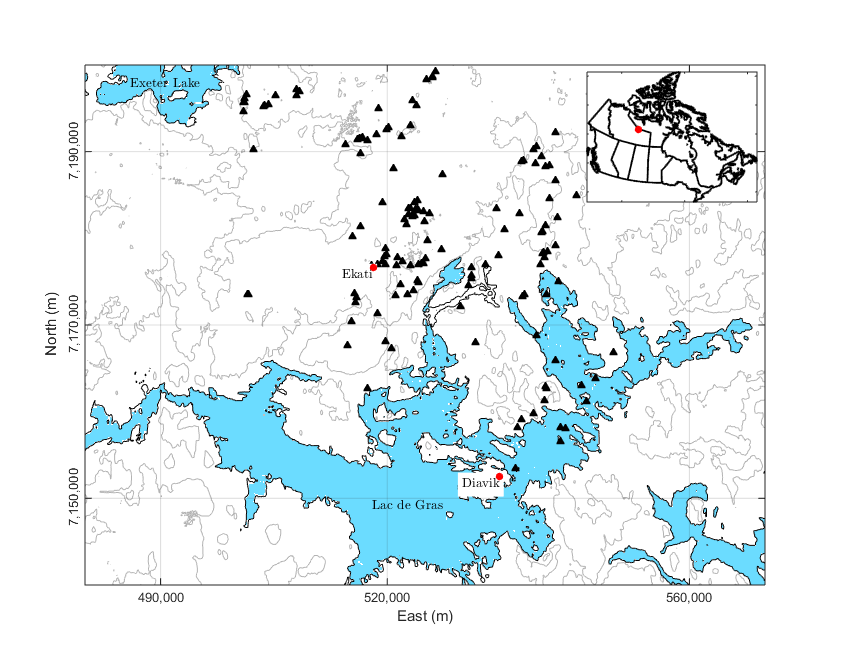
\includegraphics[scale=0.6]{Ekati_Location.png}
\caption{Topography and known kimberlites over the Lac de Gras region. The location of the main operations for the Ekati and Diavik mines are shown (red dot).}
\label{fig:Ekati_Location}
\end{figure}

\subsection{Geology}
The Lac de Gras kimberlite field is located in the Slave craton,  which consists mainly of granitoid and meta-sediment rocks dated between 2.66-2.58 Ga-old \cite[]{Creaser2004}.
The region is intruded by several phases of diabase dyke swarms clearly visible on the airborne magnetic data.
Table \ref{tbl:Dykes} summarizes the age and trend of five important groups of dykes \cite[]{Buchan09}.
It has been argued that the dykes may serve as structural control for kimberlites \cite[]{Wright1999}.


\begin{table}
\centering
\caption{Dyke swarms of the Lac de Gras region listed in increasing age as published by \cite{Buchan09}}
\label{tbl:Dykes}
\renewcommand{\arraystretch}{1.2}
\begin{tabular}{|c|c|c|}
Name & Orientation ($^\circ$) & Age (Ma) \\
Mackenzie & 315 & 1267 \\
$'305'$ & 305 & - \\
Lac de Gras & 0 & 2027-2023 \\
MacKay & 90 & 2210 \\
Malley & 45 & 2230
\end{tabular}
\end{table}


Kimberlite pipes in the Lac de Gras region are narrow, steeply sided inverted cones, with the majority of them covering less than 5 ha at the surface.
The standard model for kimberlites in the Lac de Gras region is a mix of fragmented crater facies and non-fragmented hypabyssal (HK) facies.
The crater facies in the upper portion of the type can be further subdivided in various types of volcaniclastic (VK) and pyroclastic (PK) units \cite[]{Pell1997}.
Found at greater depths, the HK unit is a coherent olivine-rich rock, and is also found as intrusive dykes and sills.
The composition and physical properties of kimberlites can vary greatly between pipes.
Geophysically, it has been found that crater facies are generally associated with density and magnetic susceptibility lows.
Weathering of the crater facies may also appear as resistivity lows due to the abundance of clay minerals, although they can easily be confounded with fine grained glaciofluvial sediments in northern regions \cite[]{PowerHildes2007}.
The hypabyssal facies on the other hand are mostly associated with magnetic susceptibility highs and are prone to retaining remanent magnetization.

Fossil bearing xenoliths in some pipes are indicative of a sub-marine emplacement between the Late Cretaceous to Eocene time.
Radiometric dating of 36 pipes indicates a wide range of emplacement times \cite[]{Creaser2004}, divided into five temporally discrete episodes \cite[]{Lockhart2004}. Three of the most productive kimberlites at Ekati (Koala, Koala North and Panda pipes) were emplaced 53 Ma ago during the Panda Age Array (PAA).
Physical property measurements of the rocks were also acquired over the Lac de Gras region and are summarized in \cite[]{Enkin2003, Buchan09}.
It has been suggested that the orientation of magnetization could be used to determine the age of a kimberlite pipe, hence it could be used to estimate the economic potential of a deposit \cite[]{Lockhart2004}.

\subsection{Airborne magnetic data}
In 1993, a fixed-wing magnetic survey was flown over the Ekati Property as shown in Figure \ref{fig:Aeromag_Location}.
The $''Paul's\;Lake''$ aeromagnetic data were downloaded from the Natural Resources Canada's website.
The data set consists of 91 survey lines of Total Magnetic Field (TMI) measurements, spaced 250 m apart, covering an area of $23\times36$ km.
Observations were provided at a 50 m spacing along line, at an average flight height of 120 m, as measured by radar altimeter.
From historical geomagnetic data, the inducing field strength was 60,275 nT, [I: $27^{\circ}$, D: $84^{\circ}$].

A Digital Elevation Model (DEM) was downloaded from the Canadian Digital Elevation Data collection (1:50,000), also provided by Natural Resources Canada.
The DEM was used to convert the radar height to absolute elevation referenced to mean sea level.

\begin{figure}[h!]
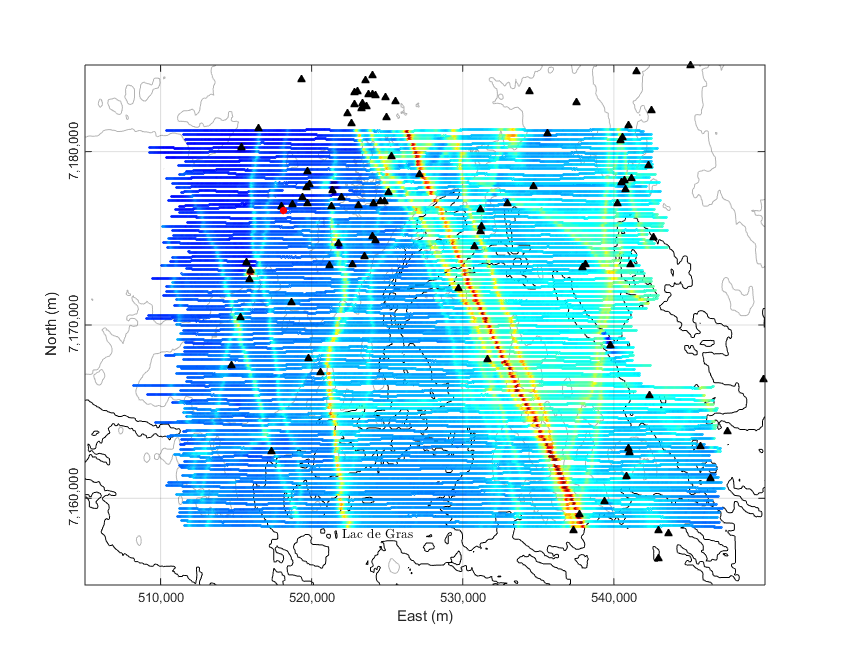
\includegraphics[scale=0.6]{Aeromag_Location.png}
\caption{Topography, aeromagnetic survey and known kimberlites over the Lac de Gras region. The location of the main operations for the Ekati and Diavik mines is marked with a red dot.}
\label{fig:Aeromag_Location}
\end{figure}


\section{Regional scale inversion}
The inversion procedure follows the methodology presented in Chapter \ref{ch:Chap5_Cooperative_Mag_Inversion_CMI}.
The objective of a regional scale inversion is to first gain knowledge about the general distribution of magnetic anomalies.
Moreover, this step is used to estimate uncertainties and to identify regions of interest for a deposit-scale inversion.

Prior to the inversion, I remove a regional trend in the data in order to focus the inversion on local anomalies. Small regions 1 $km^2$ showing low variations in the field were manually chosen as shown in Figure~\ref{fig:Ekati_Detrend_Data}(a). Within each region, the median data value and horizontal location are recorded. Those values are then used to create a first-order polynomial (Fig-\ref{fig:Ekati_Detrend_Data}(b)). A regional trend of roughly 250 nT trending up towards east is subtracted as shown in Figure~\ref{fig:Ekati_Detrend_Data}(c). I assign five percent uncertainties, plus 5 nT floor uncertainty to the data.   

\begin{figure}[h!]
\centering
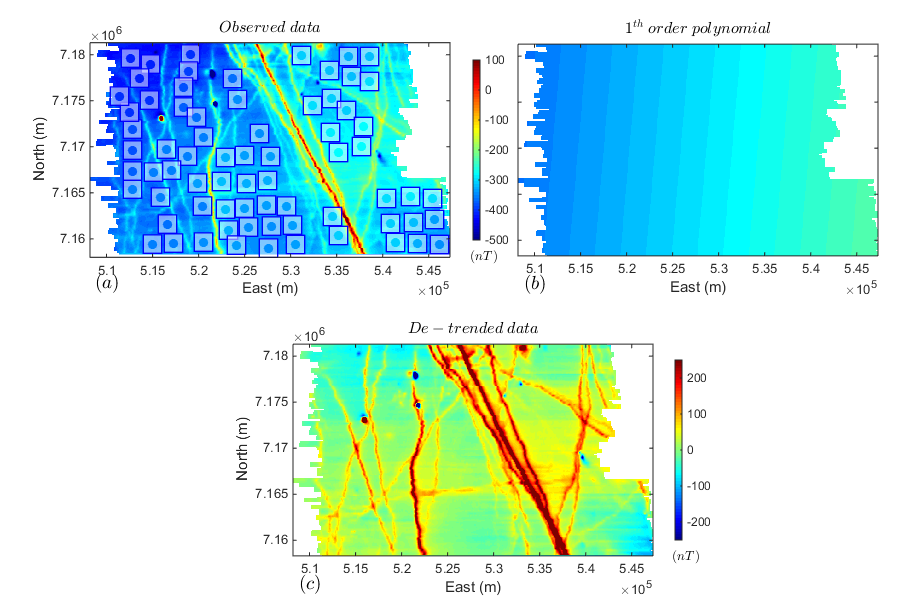
\includegraphics[scale=0.55, trim= 1cm 0 0 0]{Ekati_Detrend_Data.png}
\caption{Regional data (a) before and (c) after removal of a regional trend. The median value within selected regions (boxes) were used to compute (b) a first-order polynomial trend.}
\label{fig:Ekati_Detrend_Data}
\end{figure}

Table \ref{tbl:Reg_inv} presents some of the parameters used for the inversion.
The model space is discretized by a 50 m cell size resolution.
The depth extent of the mesh covers the top 1 km below topography,  for a base mesh of 6 M cells.
Inversion of the entire data set, approximately 50,000 observations, at this resolution remains computationally challenging for most computers.
In order to reduce the computational cost, I designed a tiled inversion procedure. Figure \ref{fig:Ekati_Tiles} presents the tiling configuration with respect to the data set.
Neighboring regions overlap by 500 m in order to share a minimum of two survey lines, guaranteeing good lateral continuity.
The procedure is readily parallelized across multiple processors, each inverting a subset of the problem independently.
The final magnetization model is interpolated onto the base mesh using a weighted average scheme such that:

\begin{equation}\label{merge}
\begin{split}
m_i &= \frac{\sum_{j=t}^T m_i^{(j)} \; w_i^{(j)}}{\sum_{j=t}^T w_i^{(j)}} \\
w_i^{(j)} & = {\Big[ { (x_i - x_c^{(j)})}^2 + { (y_i - y_c^{(j)})}^2 \Big]}^{-1/2} \;,
\end{split}
\end{equation}
where the weights $w_i^{(j)}$ are inverse distance between the $i^{th}$ cell and the center location $[x_c;y_c]$ of the $j^{th}$ tile. The number of tiles T overlapping at the $i^{th}$ cell is variable depending on the horizontal location. The same weight is used for all cells vertically at the same $[x_i;y_i]$ location.

\begin{figure}[h!]
\centering
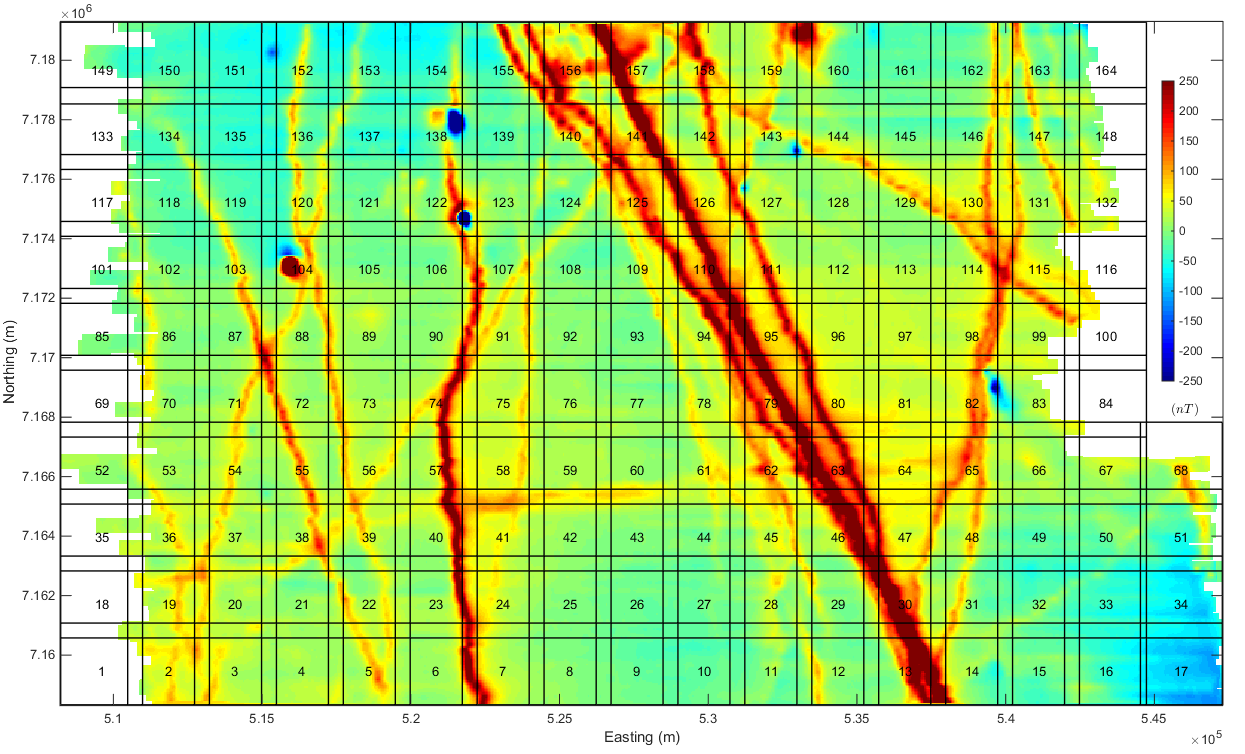
\includegraphics[scale=0.38]{Ekati_Tiles.png}
\caption{TMA data after removal of the regional signal and tiling configuration used for the regional inversion.}
\label{fig:Ekati_Tiles}
\end{figure}

\begin{table}
\centering
\caption{Regional-scale inversion parameters.}
\label{tbl:Reg_inv}
\renewcommand{\arraystretch}{1.2}
\begin{tabular}{|c|c|}
Core cell size & $75\times75\times50$ m \\
Base mesh size & 3.3 M cells \\
Number of tiles & 77 \\
M / tile & $\approx$ 100k cells \\
N / tile & $\approx$ 900 data \\
$p,\;qx,\;qy,\;qz$ & 1, 1, 1, 1 \\
$\alpha_s,\; \alpha_x,\; \alpha_y, \; \alpha_z$ & 1.8e-4, 1, 1, 1 \\
Uncertainties & 0.05*d + 5 nT
\end{tabular}
\end{table}

Figure \ref{fig:Ekati_Reg_Interp} presents a horizontal section at $\approx$50 m depth through the recovered effective susceptibility model.
As expected from the observed data, several long and narrow anomalies are recovered.
Based on the analysis by \cite{Buchan09}, I interpret the linear trends as regional dyke swarms belonging to the Mackenzie, Lac de Gras, MacKay and Malley groups.
A large number of kimberlite pipes show as effective susceptibility highs, with few exceptions.
The three Koala pipes, for example, west of the Grizzly pipe, were not well recovered.
Although important economically, the anomalous magnetic response from the pipe is below the noise level.
Proper imaging of the deposits would require a magnetic survey at lower elevation to increase the noise to signal ratio.

I note the clustering of kimberlite pipes near the intersection and along some of the dyke swarms.
The apparent correlation between kimberlite pipes and dykes seems to reinforce the idea of structural controls as put forward by \cite{Wright1999}.
While the topic is beyond the scope of this Masters thesis, future work in structural geology over the region may benefit from a regional scale inversion as presented here.

Figure~\ref{fig:Ekati_reg_Obs_Pred} compares the observed and predicted data from the tiled inversion. In the left panel, the predicted data from individual tiles were merged following \ref{merge}. The normalized residual data show horizontal striations due to variations in magnetic data between adjacent lines, which could not be accounted for by the inversion. 
Overall, each invividual inversion could predict the data well within the assigned uncertainties.
On the other hand, the right panel shows the predicted data from the final merged susceptibility model.
I here notice that some of the low frequency content has been lost during the merging process, with higher residuals over the regions of low magnetic fields.
This can be a problem when attempting to image regional features and will require further research.
In this case, we are only interested in the dykes and kimberlite pipes, which for the most part were well recovered.

\begin{figure}[h!]
\centering
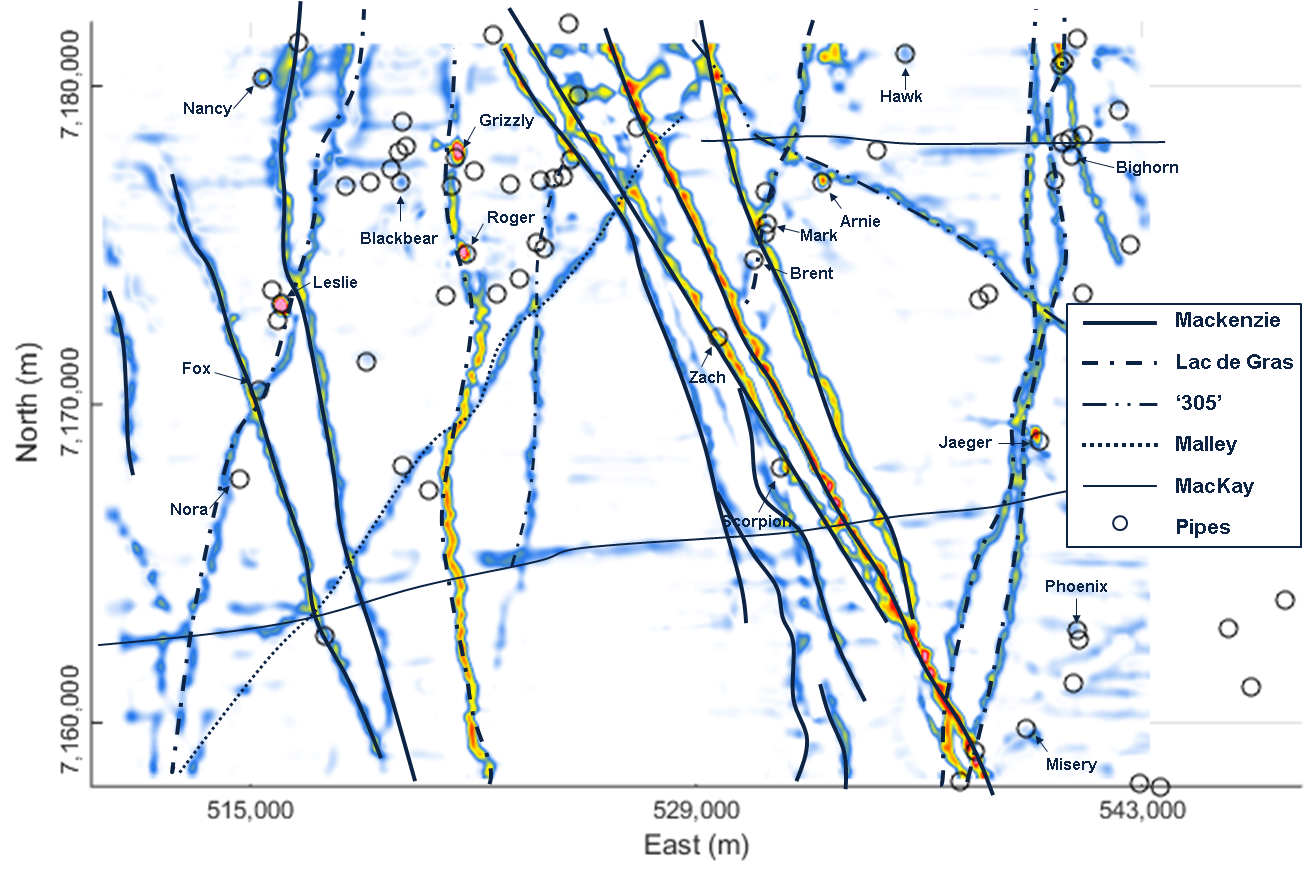
\includegraphics[scale=0.58, trim= 0.5cm 0 0 0]{Ekati_Reg_geology_interp.png}
\caption{Interpreted dykes (line) from the property-scale magnetization inversion and known kimberlite pipes location (circle). The 16 pipes chosen for a deposit-scale inversion are labeled.}
\label{fig:Ekati_Reg_Interp}
\end{figure}

\begin{figure}[h!]
\centering
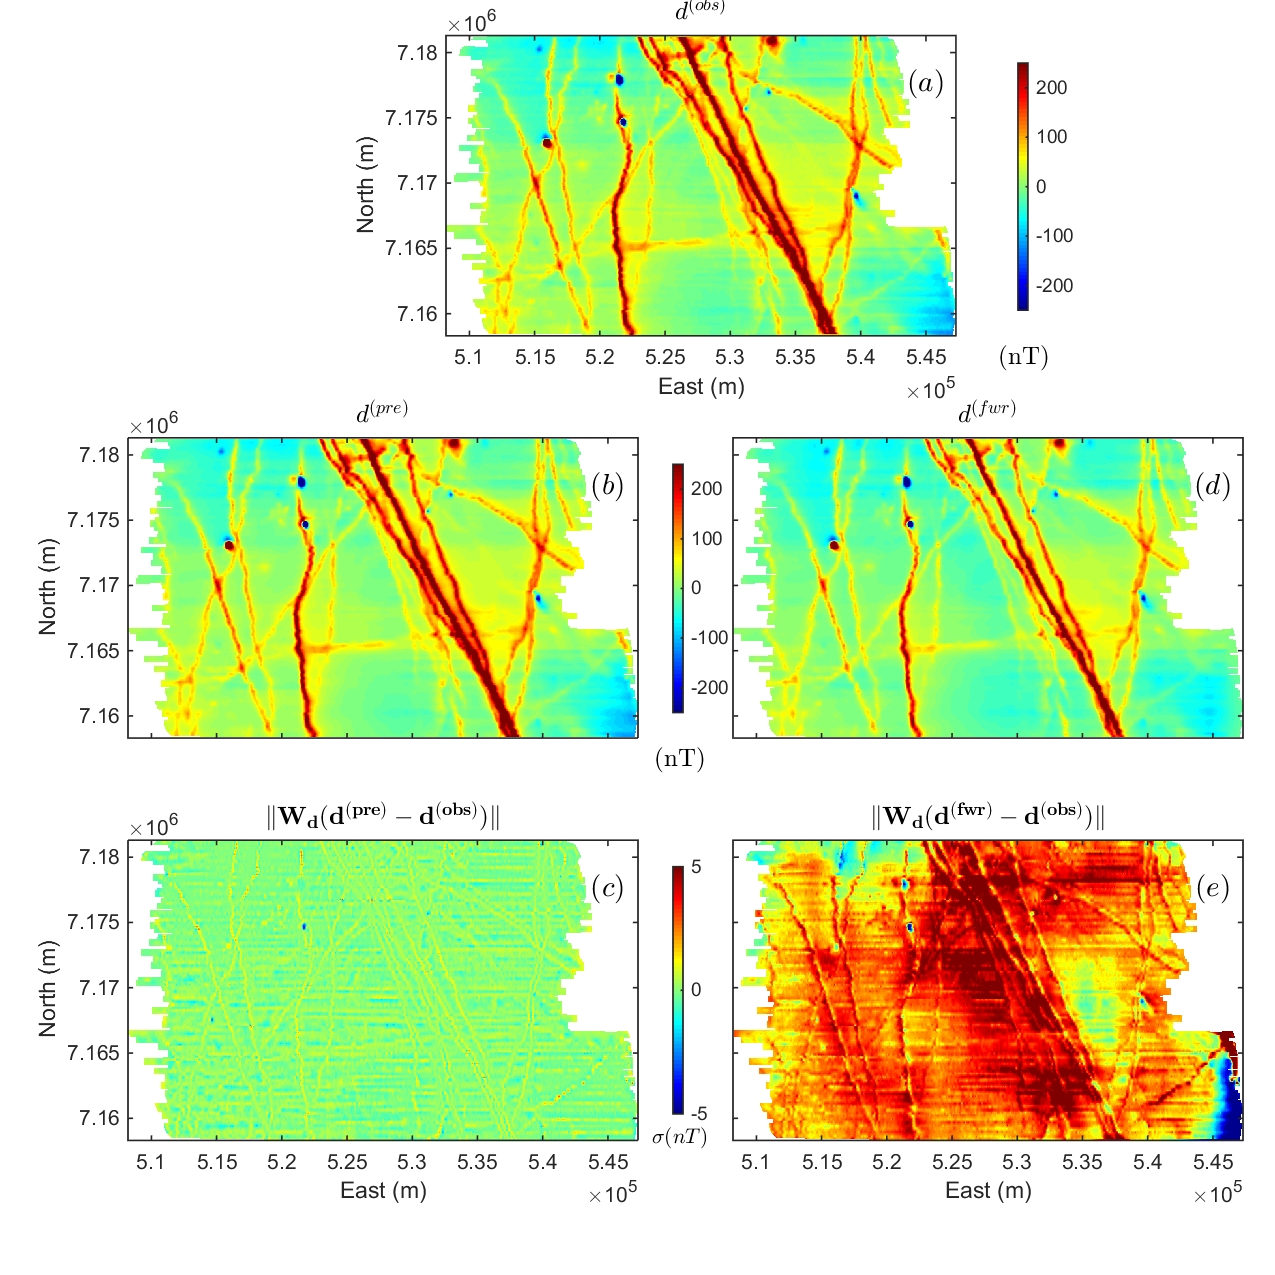
\includegraphics[scale=0.6, trim=0.75cm 0 0 0]{Ekati_reg_Obs_Pred}
\caption{Comparison between (a) observed and (b) merged predicted data from the recovered magnetization model over the Ekati Property. (c) Normalized residual data show horizontal striations due to variations in magnetic data between adjacent lines, which could not be accounted for by the inversion. Most of the predicted data from the individual tiles can fit the observed data within one standard deviation. (d) Forward modeled data from the merged magnetization model and (c) normalized data residual. It appears that a large portion of the the low frequency content has been lost during the merging step. More research is required in order to preserve the long wavelength information.}
\label{fig:Ekati_reg_Obs_Pred}
\end{figure}

\section{Deposit scale inversion}
From the property scale inversion, 16 sites were chosen based on the strength of the magnetic anomaly for a high resolution inversion.
The goal of this section is to gain knowledge about the bulk magnetization direction and compare those values to physical property measurements published in the literature.

For each inversion, a regional field was removed in order to focus the inversion on the local anomalies.
Description of the regional field removal method can be found in \cite{LiRegRem1998}.
In summary, the following steps were taken:
\begin{itemize}
\item Creation of a local mesh with large padding cells
\item Inversion of the data assuming induced magnetization
\item Removal of the local source within the core mesh. Only susceptible material outside the core region remain.
\item Forward modeling of the regional data at the observation location
\item Subtraction of the regional signal from the observed data
\end{itemize}
The regional-removal step is important in regions where the regional field is larger than the local anomaly.
Figure \ref{fig:RegRem_Misery} presents the magnetic data before and after removal of the regional field over the Misery pipe.
Note that the original data are trending up towards the east, with the largest magnetic field data occurring near the edge of the dataset. Consequently, the magnetic amplitude inversion would be biased towards having a ring of effective susceptibility around the edge of the dataset, rather than the pipe itself. 
After removing the regional field, most of the anomalous fields come from a strong negative anomaly corresponding with the location of the Misery pipe.

\begin{figure}[h]
\centering
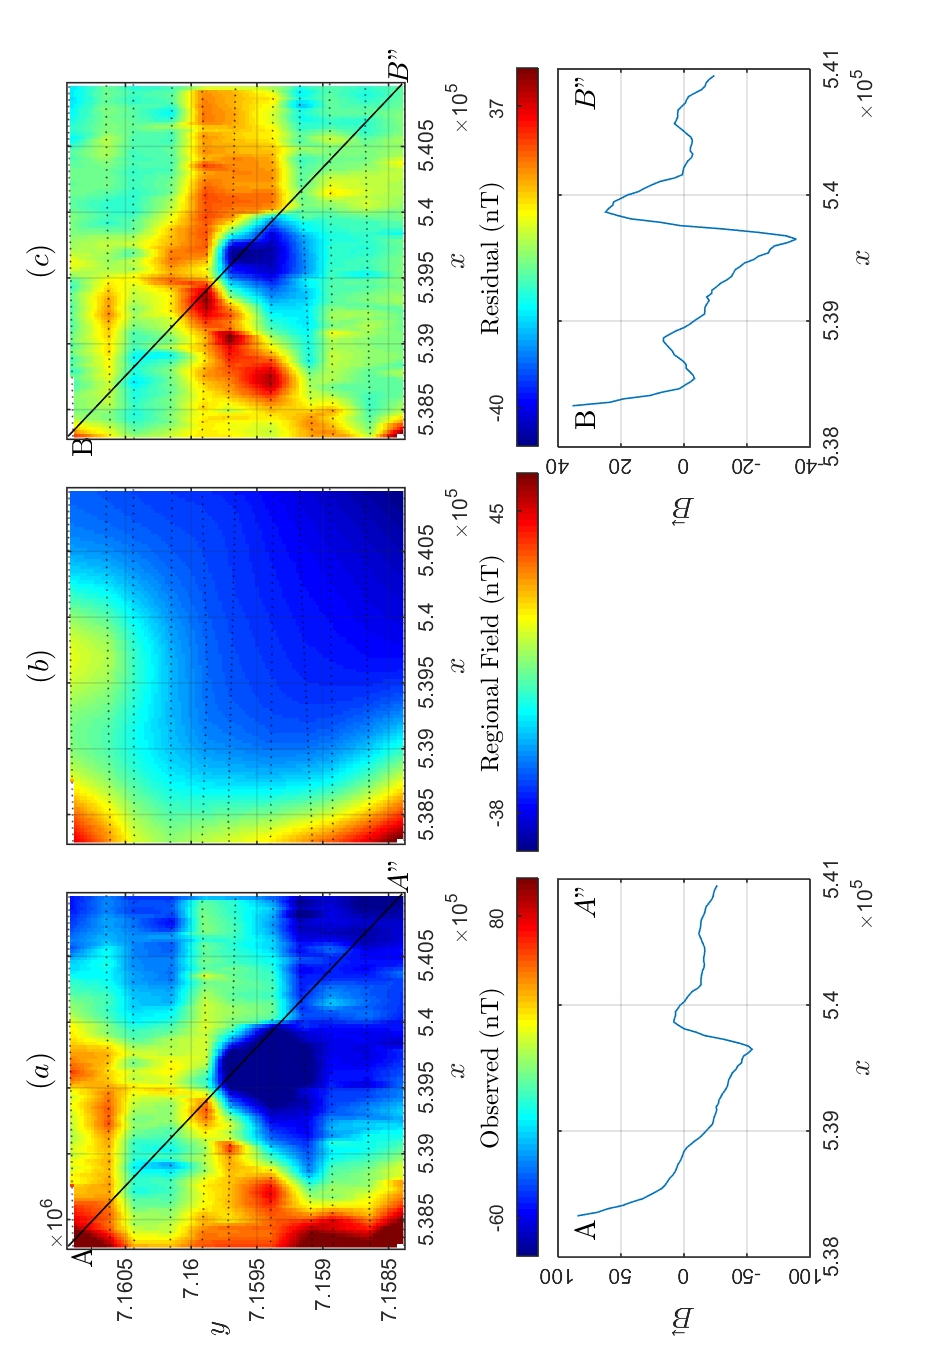
\includegraphics[scale=0.55,angle=270]{RegRem_Misery}
\caption{(a) Local data collected over the Misery pipe showing a local western trend. (b) Regional field data are computed from a local inversion. Most of the signal comes from a dyke running north-south along the western edge of the local tile. (c) Residual data after regional field removal, showing a clear reversely magnetized anomalie corresponding with the location of the Misery pipe.}
\label{fig:RegRem_Misery}
\end{figure}

Following the regional field removal, each local tile is inverted with the CMI algorithm on a 25 m cell size mesh.
This resolution is required in order to properly model narrow anomalies in the range of 50 to 100 m in width.
The process was repeated for the selected 16 kimberlite pipes.
Table \ref{tbl:Dep_inv} summarizes the parameters used for the inversions.
I imposed an $l_0$-norm on the amplitude of magnetization in order to focus the inversion within the core of the different kimberlites pipes. The direction of magnetization was allowed to vary smoothly in order to get an estimate of the variability, and hence to get a measure of uncertainty. A 27 point average (3x3x3 cells) centered over the location of each pipe was used to compute an effective susceptibility and direction as shown in Table \ref{Local_Summary}.
In the following section, the results are compared to those published in the literature.


\begin{table}
\centering
\caption{Deposit-scale inversion parameters.}
\label{tbl:Dep_inv}
\renewcommand{\arraystretch}{1.2}
\begin{tabular}{|c|c|}\hline
Core cell size & $25\times25\times25$ m \\
Base mesh size & 50 M cells \\
Number of tiles & 17 \\
M / tile & $\approx$ 200k cells \\
N / tile & $\approx$ 150 data \\
$p,\;qx,\;qy,\;qz$ & 0, 2, 2, 2 \\
$\alpha_s,\; \alpha_x,\; \alpha_y, \; \alpha_z$ & 1.6e-3, 1, 1, 1 \\
Uncertainties & 0.02*d + 5 nT \\ \hline
\end{tabular}
\end{table}
\begin{table}[]
\centering
\caption{Average magnetization amplitude and direction from the local inversion over 16 known kimberlite pipes. Uncertainties were calculated from a three-cell cube standard deviation around the approximate location of each kimberlite pipe.}
\label{Local_Summary}
\renewcommand{\arraystretch}{1.}
\begin{tabular}{|c|c|c|c|c|c|}\hline
Pipe ID &	X (m) &	Y (m) &	$\kappa_{e}$ &	Incl ($^{\circ}$) &	Decl ($^{\circ}$) \\ \hline
Arnie &	532980 &	7176930 &	3.9e-2 $\pm$ 1.0e-2 &	 -85 $\pm$ 4.2 &	 355 $\pm$ 5.0 \\
Blackbear &	519700 &	7176980 &	9.9e-4 $\pm$ 1.3e-4 &	 -88 $\pm$ 1.9 &	 211 $\pm$ 3.0 \\
Brent &	530855 &	7174206 &	4.6e-3 $\pm$ 2.0e-3 &	 -79 $\pm$ 3.1 &	 299 $\pm$ 2.3 \\
Fox &	515091 &	7169946 &	2.4e-2 $\pm$ 8.0e-3 &	 66 $\pm$ 17.7 &	 203 $\pm$14.9 \\
Grizzly &	521529 &	7177946 &	8.7e-2 $\pm$ 8.6e-3 &	 -82 $\pm$ 1.3 &	 100 $\pm$ 1.7 \\
Hawk &	535550 &	7180934 &	2.0e-3 $\pm$ 1.6e-4 &	 -84 $\pm$ 0.2 &	 244 $\pm$ 0.1 \\
Jaeger &	539575 &	7168970 &	2.3e-2 $\pm$ 6.6e-3 &	 -73 $\pm$ 2.6 &	 53 $\pm$ 2.8 \\
Leslie &	515960 &	7173130 &	3.6e-1 $\pm$ 6.0e-2 &	 65 $\pm$ 3.7 &	 346 $\pm$ 5.2 \\
Mark &	531202 &	7175715 &	4.5e-2 $\pm$ 7.0e-3 &	 -83 $\pm$ 4.0 &	 159 $\pm$ 5.4 \\
Nancy &	515351 &	7180271 &	1.0e-2 $\pm$ 8.0e-4 &	 -84 $\pm$ 2.1 &	 11 $\pm$ 2.0 \\
Nora &	514665 &	7167532 &	2.0e-3 $\pm$ 2.6e-4 &	 -87 $\pm$ 2.1 &	 287 $\pm$ 4.3 \\
Phoenix &	540829 &	7162932 &	1.5e-4 $\pm$ 2.1e-5 &	 -85 $\pm$ 1.8 &	 238 $\pm$ 1.3 \\
Roger &	521770 &	7174655 &	1.3e+0 $\pm$ 4.2e-1 &	 -82 $\pm$ 5.3 &	 160 $\pm$ 10.9 \\
Scorpion &	531854 &	7167847 &	2.5e-2 $\pm$ 1.1e-2 &	 68 $\pm$ 13.0 &	 258 $\pm$ 23.6 \\
Zach &	529812 &	7171900 &	3.4e-2 $\pm$ 8.8e-3 &	 82 $\pm$ 7.9 &	 185 $\pm$ 9.4 \\
Misery &	539621 &	7159630 &	7.3e-3 $\pm$ 1.3e-3 &	 -77 $\pm$ 5.0 &	 172 $\pm$ 10.1 \\ \hline
\end{tabular}
\end{table}

\section{Discussion}
Magnetization inversion at a regional scale reveals interesting patterns.
Figure \ref{fig:Ekati_reg_IND_REM} compares the induced and remanent components of magnetization over the property.
The remanent component is noticeably stronger on most of the NE trending Mackenzie dykes, while the Lac de Gras and MacKay dykes seem to be mainly magnetized along the inducing field.
Several points of intersection between the Lac de Gras, Mackenzie and Malley dykes in the south of survey [537,000 E ; 7,176,000 N] show a strong remanent component.
This result seems to agree with the study of \cite{Buchan09}.
The low resolution of this airborne survey does not support accurate modeling of narrow dykes on the order of 10 to 30 m width.
It can however provide a relative time of emplacement when comparing the strength and trend of effective susceptibility of intersecting dykes.
Note the clear magnetic overprinting of a NW trending dyke onto a NE dyke near the Fox pipe [515,000 E ; 7,170,000 N] and Leslie pipe [516,600 E ; 7,174,000 N].
This result fits with the idea of a younger Mackenzie dyke swarm (1270 Ma) crosscutting an older Lac de Gras dyke (2020 Ma).

Note that the NS trending dyke intercepting the Grizzly pipe has been recovered on its entire length with a relatively strong induced component. This is despite the large footprint of a reversely magnetized body, which illustrates the strength of the CMI algorithm in its ability to distinguish between adjacent anomalies with varying magnetic orientations.


\begin{figure}[p]
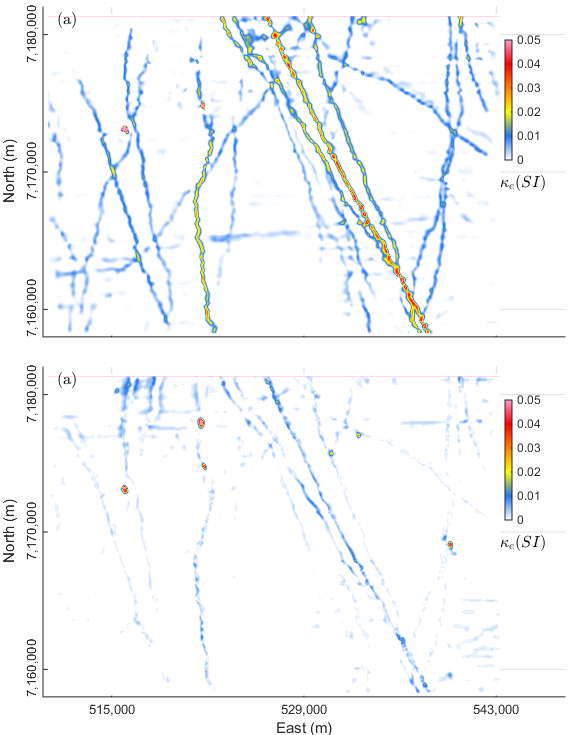
\includegraphics[scale=0.8]{Ekati_reg_IND_REM.png}
\caption{Horizontal sections through the recovered (a) induced and (b) remanent magnetization model. Several pipes with strong remanence can easily be identified as discrete circular anomalies.}
\label{fig:Ekati_reg_IND_REM}
\end{figure}

Several of the 16 pipes have been studied in the past, some of which have borehole samples measured in laboratory.
Table \ref{Published_Summary} summarizes the information collected from the literature.
In general terms, my results seem to agree more with \cite{Enkin2003} and \cite{Cheman2006} in terms of orientation compared to the results of \cite{Zhao2012}.
It is important to point out that the inversion results offer a bulk estimate of magnetization within the pipe, which are known to be highly heterogeneous. Laboratory measurements provided by \cite{Enkin2003} showed large variations in magnetic properties along individual boreholes.
Moreover, larger uncertainties are expected from the recovered declination in cases where the magnetization vector is nearly vertical ($I > 80^{\circ}$).

Finally, I analyze the age of the kimberlite pipes in relation to the magnetization direction.
Table \ref{Age_Summary} summarizes the age group as identified by \cite{Lockhart2004}, as well as the predicted polarity from the geomagnetic timescale provided by \cite{Cande1995}.
Figure~\ref{fig:Ekati_Pipe_time} maps on a timescale the polarity of the various pipes with respect to Earth's polarity reversal.
It is interesting to note that several of the predicted polarity directions from radiometric dating do not agree with the recovered polarity.
Those differences could be a result of uncertainties in the Rb-Sr radiometric dating of $\pm1$ Ma (2$\sigma$).

It is important to note the frequent changes in Earth's polarity during the period of 46 and 69 Ma, with at least 14 reversals identified.
My results seem to suggest that the age array MAA should be between 48 and 49 Ma in order to account for the recovered negative polarity.
Similarly, the Leslie pipe should be either younger than 51.7 or older than 52.7 to be normally magnetized.
The Roger pipe is particularly interesting as it is clearly reversely magnetized, and could have only been formed during the short time window of 67.61 to 67.73 Ma.

As suggested by \cite{Lockhart2004}, the microdiamond abundance of kimberlite pipes observed at Ekati may be correlated in time.
It has been found however that the magmatism can vary greatly between each eruption episode, even if all episodes occur in close spatial proximity.
Future research could look into correlations between magnetization strength and direction, as well as electrical properties of the different pipes.
Assuming that diamond grade and abundance are related to the mantle source, it can be expected that rock magnetic susceptibility and electrical conductivity would be a better proxy for diamond content than age of emplacement.
High resolution magnetic and airborne EM inversions could lead to interesting insights into the Ekati property.


\begin{table}[]
\centering
\caption{Summary of published results over selected kimberlite pipes}
\label{Published_Summary}
\renewcommand{\arraystretch}{1.1}
\begin{tabular}{|c|c|c|c|}\hline
\multirow{2}{*}{Source} & Leslie & Misery & Grizzly \\
& $I^{\circ} | D^{\circ}$ & $I^{\circ} | D^{\circ}$ & $I^{\circ} | D^{\circ}$ \\
\hline
CMI & \begin{tabular}{c c} 65 & 346 \end{tabular} & \begin{tabular}{c c} -77 & 172 \end{tabular} & \begin{tabular}{c c} -82 & 100 \end{tabular} \\
\cite{Enkin2003} & \begin{tabular}{c c} 64 & 329 \end{tabular} & \begin{tabular}{c c} -74 & 168 \end{tabular} & *** \\
\cite{Zhao2012} & \begin{tabular}{c c} 59 & 334 \end{tabular} & *** & \begin{tabular}{c c} -58 & 316 \end{tabular} \\
\cite{Cheman2006} & \begin{tabular}{c c} 82 & *** \end{tabular} & *** & \begin{tabular}{c c} -73 & *** \end{tabular} \\ \hline
\end{tabular}
\end{table}

\begin{figure}[h!]
\centering
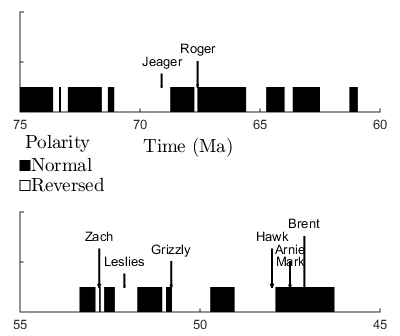
\includegraphics[scale=0.8]{Ekati_Pipe_time.png}
\caption{Age of 11 pipes from the Ekati region with respect to Earth's polarity reversal.}
\label{fig:Ekati_Pipe_time}
\end{figure}


\begin{table}[]
\centering
\caption{Radiometric age and inverted magnetization direction for 11 pipes.}
\label{Age_Summary}
\renewcommand{\arraystretch}{1.2}
\begin{tabular}{|c|c|c|c|c|c|c|}
\hline
	\multirow{2}{*}{Pipe ID} 	&	Age Array &	Age &	\multirow{2}{*}{Polarity Chron} 	&	Incl &	Decl \\
						&	\cite{Lockhart2004}	& (Ma)	& (+ , - )	& $(^{\circ})$ & $(^{\circ})$ \\
	\hline
	Brent 	&	\multirow{4}{*}{MAA}		&47.1 &	C21n (+) 	&	 -79.0 $\pm$ 3.1 &	 299.0 $\pm$ 2.3 \\
	Arnie 	&	&47.5 &	C21n (+) 	&	 -85.9 $\pm$ 4.2 &	 355.5 $\pm$ 5.0 \\
	Mark 	&	&47.5 &	C21n (+) 	&	 -83.9 $\pm$ 4.0 &	 159.1 $\pm$ 5.4 \\
	Hawk 	&	&48.0 &	(-) &	 -84.3 $\pm$ 0.2 &	 244.4 $\pm$ 0.1 \\
	\hline
	Grizzly 	&	&50.8 &	C23n.1n (+) 	&	 -82.2 $\pm$ 1.3 &	 100.1 $\pm$ 1.7 \\ \hline
	Leslie 	&	\multirow{2}{*}{PAA}&52.1 &	(-) &	 65.4 $\pm$ 3.7 &	 346.3 $\pm$ 5.2 \\
	Zach 	&	&52.8 &	C24n.2n (+) 	&	 82.5 $\pm$ 7.9 &	 185.8 $\pm$ 9.4 \\
	\hline
	Roger 	&	\multirow{2}{*}{MSK}&67.6 &	C30n (+) 	&	 -82.7 $\pm$ 5.3 &	 160.1 $\pm$ 10.9 \\
	Jaeger 	&	&69.1 &	(-) &	 -73.2 $\pm$ 2.6 &	 53.2 $\pm$ 2.8 \\
	\hline
	Nora 	&	&2106 & 	- 		&	 -87.4 $\pm$ 2.1 &	 287.9 $\pm$ 4.3 \\
	Misery 	&	&2480 & 	- 		&	 -77.6 $\pm$ 5.0 &	 172.3 $\pm$ 10.1 \\ \hline
	
\end{tabular}

\end{table}


\endinput


